\chapter{Introdução}
\label{cha:introducao}

A idéia de preservação de contorno e variação de intervalos entre
notas é encontrada em diferentes situações musicais. Há adequação de
notas à tonalidade em respostas tonais de fugas, em mudanças de modo
em peças do tipo tema e variações, e em \eng{leitmotifs} e idéias
fixas, citando apenas exemplos óbvios
\cite[p. 29]{morris87:composition}. Outras obras têm motivos cujos
intervalos são pouco a pouco expandidos ou contraídos, como por
exemplo ocorre no início da \opus{Música para Cordas, Percussão e
  Celesta}, de Béla Bartók.

Teóricos musicais reconhecem que ouvintes têm maior acuidade na
percepção de semelhança de contornos do que na semelhança de
alturas. Por isso novas teorias para comparação de contornos se
tornaram necessárias à área da Análise Musical
\cite[p. 226]{marvin.ea87:relating}.

\chapter{Sobre contornos}
\label{cha:sobre-contornos}

%% brainstorm

% análise: comparação e equivalência de materiais.
% análise: objetivos diferentes.
% redução: tipologia de adams e algoritmo de morris
% equivalência a partir de matriz de comparação
% cognição: dowling
% terminologias diferentes: friedmann
% problemas com teorias: clifford
% estruturação da composição a partir de contornos
% exemplos com análise de peças?
% contornos: coerência, schoenberg

%% lembrete: falar que não abordaremos o aspecto duração

Teorias de contornos foram desenvolvidas primariamente como técnicas
analíticas para composições atonais que podem não ter características
musicais usadas para demonstrar coerência em composições tonais
\cite[p. 1]{beard03:contour}.

Embora teorias de contorno não tenham surgido para análise de obras
tonais, a análise a partir da perspectiva dos contornos já se mostrou
eficiente também neste tipo de obra. Assim, além de obras de Schönberg
\cite{friedmann85:methodology} e Webern \cite{clifford95:contour},
sonatas para piano de Mozart \cite{beard03:contour} já foram
analisadas sob a ótica das teorias de contornos.

Contorno é um conjunto ordenado de elementos distintos, com ou sem
repetição, numerados de forma ascendente
\cite[p. 206]{morris93:directions}. Por definição contornos musicais
são ordenados \cite[p. 228]{marvin.ea87:relating}.

Um contorno pode ser interpretado como registro, dinâmica ou densidade
de acordes no tempo \cite[p. 206]{morris93:directions}
\cite[p. 22]{clifford95:contour}. Podemos ver representações do
contorno \contorno{4\:3\:5\:6} na figura
\ref{fig:non-melodic-contours}.

\begin{figure}
  \centering
  \subfloat[alturas no tempo]{
    \includegraphics[scale=1]{pitches-in-time}
    \label{fig:pitches-in-time}}
  \subfloat[densidade de acordes no tempo]{
    \includegraphics[scale=1]{chord-densities-in-time}
    \label{fig:chord-densities-in-time}}

  \subfloat[dinâmicas no tempo]{
    \includegraphics[scale=1]{dynamics-in-time}
    \label{fig:dynamics-in-time}}
  \caption{Contornos \contorno{4\:3\:5\:6} não melódicos}
  \label{fig:non-melodic-contours}
\end{figure}

Adams propôs uma tipologia de contornos melódicos para classificação
de melodias indígenas americanas. Esta tipologia está baseada na
redução do contorno de cada melodia a quatro pontos --- nota inicial
(I), nota final (F), nota mais aguda (H) e nota mais grave (L) --- e
na classificação da inclinação entre essas notas. A inclinação entre
as notas pode ser ascendente, descendente ou nula, e repetição de
notas são admitidas. Adams propôs 15 tipos de contornos melódicos,
como se vê na figura \ref{fig:adams-typology}. A inclinação (ou
\eng{slope}) entre a nota inicial e final é indicada por $S1$ ($I >
F$), $S2$ ($I = F$) e $S3$ ($I < F$). A mudança de direção (ou
\eng{deviation}) é indicada por $Dø$ (sem mudança de direção), $D1$
(se H ou L são diferentes de I ou F) e $D2$ (se H e L são diferentes
de I e F). A ordem entre as mudanças de direção, chamada
\eng{reciprocal}, é indicada por $R1$ (H antes de L) e $R2$ (L antes
de H) \cite{adams76:melodic}.

\begin{figure}
  \centering
  \includegraphics[scale=.6]{adams-typology}
  \caption{Tipologia de contornos de Charles Adams}
  \label{fig:adams-typology}
\end{figure}

A terminologia utilizada em teorias de contornos melódicos não é
uniforme. Cada autor utiliza termos diferentes para operações
semelhantes \cite{friedmann87:response}. A tabela
\ref{tab:compara-ferramentas} tem uma comparação dos termos usados por
Friedmann, e Morris, Marvin e Laprade.

\begin{table}
  \centering
  \begin{tabular}{l|l}
    Friedmann & Marvin e Laprade \\ \hline
    \eg{cas}  & $INT_1$ \\
  \end{tabular}
  \caption{Quadro comparativo de ferramentas de análise de contornos}
  \label{tab:compara-ferramentas}
\end{table}

Morris define os conceitos de espaço de alturas (\eg{p-space}) e
espaço de contorno (\eg{c-space}) \cite{morris87:composition}. Em
\eg{p-space} os elementos a serem considerados são as notas e em
\eg{c-space} os elementos são os registros dessas notas. Beard
confunde a idéia de espaço do contorno com a definição de classe de
contorno \cite[p. 11]{beard03:contour}.

A Matriz de Comparação (\eg{com-matrix}) representa o total de
comparações de um contorno. É obtida através da comparação de todos os
pares ordenados de um contorno. Em uma matriz $E$ de um contorno $P$,
a posição $E (x,y)$ contém $Com (Px,Py)$. A matriz exibe uma simetria
de sinais invertidos em torno da diagonal principal, esta preenchida
apenas por zeros. Um exemplo desta matriz referente ao contorno
$\langle 4\:3\:5\:6 \rangle$ pode ser visto na tabela
\ref{fig:matriz-4356} \cite[p. 28]{morris87:composition}.

\begin{figure}
  \centering
  \begin{tabular}{r|cccc}
    & $4$ & $3$ & $5$ & $6$ \\
    \hline
    $4$ & $0$ & $-$ & $+$ & $+$ \\
    $3$ & $+$ & $0$ & $+$ & $+$ \\
    $5$ & $-$ & $-$ & $0$ & $+$ \\
    $6$ & $-$ & $-$ & $-$ & $0$ \\
  \end{tabular}
  \caption{Matriz de comparação do contorno $\langle 4\:3\:5\:6 \rangle$}
  \label{fig:matriz-4356}
\end{figure}

Cada diagonal à direita da diagonal zero recebe o nome $INT_n$, onde
$n$ representa a diferença de posição entre dois elementos. Dessa
forma $INT_1$ representa as diferenças de altura entre \eg{cps}
adjacentes, $INT_2$ representa as diferenças de altura entre
\eng{c-pitches} separados não adjacentes separados por um elemento e
assim por diante \cite[p. 231]{marvin.ea87:relating}. Dado um contorno
$\langle 4\:3\:5\:6 \rangle$, $INT_1 = \langle - + +\rangle$
representa as diferenças entre $4$ e $3$, $3$ e $5$, e $5$ e
$6$. $INT_2 = \langle + + \rangle$ representa as diferenças entre $4$
e $5$, e $3$ e $6$.

Esta matriz permite a verificação de duas classes de equivalência de
contornos. A primeira é formada por todos os \eg{cseg} que dividem
uma mesma \eg{com-matrix}, e a segunda ---
\eg{csegclass} --- formada por todos os \eg{cseg} relacionados
por operações de identidade, translação, retrogradação, inversão e
retrogradação da inversão.

A operação de inversão é obtida pela subtração de todos os
\eg{cps} por $(n-1)$. Para um dado \eg{cseg} $P$, a
operação de identidade é identificada como $IP$. A retrogradação de um
\eg{cseg} $P$ (representado por $RP$), bem como de sua inversão
($IP$) são obtidas colocando os \eg{cps} em ordem reversa
\cite[p. 231]{marvin.ea87:relating}.

A forma prima de um \eg{cseg} é obtida operando-se de um
algoritmo de três etapas:
\begin{enumerate}
\item realiza-se a translação do \eg{cseg} caso seja necessário;
\item se a subtração de $(n-1)$ pelo último \eg{cps} é menor
  que o primeiro \eg{cps}, inverte-se a \eg{cseg};
\item se o último \eg{cps} é menor que o primeiro
  \eg{cps} retrograda-se a \eg{cseg}.
\end{enumerate}

Michael Friedmann procurou desenvolver uma metodologia para estudo
sistemático de contornos \cite{friedmann85:methodology}. Para isso
criou duas ferramentas principais:

\begin{enumerate}
\item \eg{cas} (CAS) e
\item \eg{cc} (CC).
\end{enumerate}

Há mais seis ferramentas derivadas dessas duas principais:

\begin{enumerate}
\item \eg{casv} (CASV),
\item \eg{ci} (CI),
\item \eg{cis} (CIS),
\item \eg{cia} (CIA),
\item \eg{ccvi} (CCVI), e
\item \eg{ccvii} (CCVII).
\end{enumerate}

A série de classe de contornos adjacentes é um subconjunto da matriz
de comparação representada pela diagonal superior à diagonal zero.

\section{Percepção de contornos}
\label{sec:perc-de-cont}

Contorno melódico é uma importante característica musical no
reconhecimento de melodias familiares
\cite[p. 136]{dowling.ea86:music}. Esta afirmação é endossada por
experimentos realizados por White \cite{white60:recognition}, e
Dowling e Fujitani \cite{dowling.ea71:contour} nos quais ouvintes
foram submetidos ao reconhecimento de versões de canções familiares as
quais intervalos melódicos e/ou ritmo eram modificados e o contorno
preservado.

Implicações do estudo de contornos na música do século XX são mais
significativas para os ouvintes do que para os compositores. Isto
porque a percepção de contornos é mais geral do que a percepção de
altura e dos outros elementos do universo da teoria atonal
\cite[p. 224]{friedmann85:methodology}.

A idéia de Hindemith sobre percepção de contornos é semelhante à dos
demais autores, embora o contexto em que se aplique seja o do estudo
da harmonia. De acordo com ele é mais fácil lembrar de sucessão
rítmica e de curvas de uma linha melódica do que de diferenças em
tensão entre harmonias \cite[p. 175]{hindemith41:craft}.

\section{Contorno como determinante composicional}
\label{sec:cont-como-determ}

Clifford afirma que

%%% quando citamos literalmente, é bom fazer algum comentario

\citacaolonga{contour, in absence of other pervasive systems of pitch
  organization, represents a structural factor equal in significance
  to pitch or set class relations}{contorno, na falta de outros
  sistemas ocupantes de organização de altura, representa um fator
  estrutural igual em significado a relações de alturas ou de classes
  de conjuntos}{p. 157}{clifford95:contour}

No nível melódico relações de contorno podem associar segmentos de
contorno distintos entre dois ou mais segmentos. Neste nível contorno
pode contribuir com um processo de transformação melódica
\cite[p. 159]{clifford95:contour}.

\chapter{Ferramentas}
\label{cha:ferramentas}

\chapter{Análise da composição}
\label{cha:anal-da-comp}

A obra \obra{} é um quinteto de madeiras com trompa em movimento
único. Sua composição foi focada no uso sistemático de contornos
melódicos e não-melódicos. Além do uso de contornos trabalhamos em um
nível secundário com proporções, metas composicionais, gestos e
motivos

A obra contém duas estruturas musicais a partir das quais todo o
material composicional é derivado. A primeira estrutura é uma
bifonia---representada pela figura \ref{fig:bifonia}---e a segunda é o
motivo principal da obra, representado pela figura
\ref{fig:motivo-principal}. Este motivo é derivado por meio de
alternância entre as notas das duas vozes da bifonia.

\begin{figure}
  \centering
  \subfloat [Bifonia]{
    \includegraphics{bifonia}
    \label{fig:bifonia}
  }
  \subfloat [Motivo principal]{
    \includegraphics{motivo-principal}
    \label{fig:motivo-principal}
  }
  \caption{Elementos geradores}
  \label{fig:elementos-geradores}
\end{figure}

\section{Aspectos formais}
\label{sec:aspectos-formais}

Esta obra pode ser dividida em sete seções. Cada uma destas seções
contém uma textura característica, um desenho gestual e uma meta
composicional. O tamanho de cada seção foi definido no planejamento
inicial da obra com proporções baseadas na razão áurea. Porém, como
admitimos uma tolerância relativamente alta entre planejamento e
resultado final, estas proporções ficaram diferentes na versão final
da obra. Admitimos esta alta tolerância porque decidimos concentrar
esforços no objetivo principal do trabalho. Dessa forma deixamos
questões como as proporções formais em segundo plano.

A tabela \ref{tab:secoes-obra} contém informações de cada uma das
seções da obra como a duração, andamento, a localização do seu início
e fim pelo número de compasso e letra de ensaio.

\begin{table}
  \centering
  \begin{tabular}{r|ccccccc}
    Seção & 1 & 2 & 3 & 4 & 5 & 6 & 7 \\
    \hline
    Início (letra ensaio) & - & E & H & L & O & R & U \\
    Início (comp.) & 1 & 37 & 57 & 105 & 134 & 173 & 215 \\
    Final (comp.) & 36 & 56 & 104 & 133 & 172 & 214 & 244 \\
    Duração aprox. (s) & 132 & 91 & 108 & 56 & 87 & 23 & 16\\
    Andamento M.M & 82 & 66 & 120 & 120 & 108 & 112 & 112 \\
  \end{tabular}
  \caption{Seções formais da obra}
  \label{tab:secoes-obra}
\end{table}

\section{Aspectos verticais}
\label{sec:aspectos-verticais}
%% aspectos "harmônicos". melhorar título da seção

A bifonia (figura \ref{fig:bifonia}) que origina todo material da peça
tem seu conteúdo harmônico derivado da escala octatônica (figura
\ref{fig:escala-octatonica}).

\begin{figure}
  \centering
  \includegraphics{escala-octatonica}
  \caption{Escala octatônica}
  \label{fig:escala-octatonica}
\end{figure}

Ao longo da obra um acorde é apresentado de forma recorrente (vide
figura \ref{fig:acorde-motivo}). Este acorde é derivado da bifonia e
tem sonoridade octatônica. A terceira seção da peça é inteiramente
construída com este acorde, que tem sua orquestração modificada no
decorrer do gesto.

\begin{figure}
  \centering
  \includegraphics{acorde-motivo}
  \caption{Acorde-motivo}
  \label{fig:acorde-motivo}
\end{figure}

\section{Uso de motivos}
\label{sec:uso-de-motivos}

A obra contém motivos derivados da bifonia (vide figura
\ref{fig:bifonia}). O motivo principal da peça (vide figura
\ref{fig:motivo-principal}) dá origem aos motivos de três notas e de
semicolcheias apresentados na figura \ref{fig:motivo-3-notas}.

\begin{figure}
  \centering
  \subfloat[Motivo de três notas]{
    \includegraphics{motivo-3-notas}
    \label{fig:motivo-3-notas}
  }
  \subfloat[Motivo de semicolcheias]{
    \includegraphics{motivo-semicolcheias}
    \label{fig:motivo-semicolcheias}
  }
  \caption{Motivos utilizados na obra}
  \label{fig:motivos-utilizados}
\end{figure}

O motivo principal da peça contém dois motivos de três notas, um em
sua forma original e outro invertido. Além disso ele também está
presente de forma invertida no motivo de semicolcheias, com as notas
$C$-$E\flat$-$D\flat$. Este motivo é utilizado na linha do fagote do
início da peça, no sujeito do fugato da quarta seção (letra L), na
linha do clarinete nos compassos 137--144, na linha da flauta nos
compassos 158--171, no material da flauta e oboé na sexta seção (letra
R) e na seção final (vide seção )
%% inserir figura com linha inicial do fagote
%% inserir seção em que falo que a última seção é resumo das outras

O motivo de semicolcheias é exatamente um retrógrado do motivo
principal com a adição do parâmetro duração e da característica
anacrúzica. O motivo Está presente na linha do oboé, compasso 149, nas
linhas da flauta e clarinete nos compassos 157--172, na contrução do
material ascendente dos compassos 200--215 e na seção final.

O motivo rítmico não tem relação com altura ou contorno. É apenas um
padrão de acentuação que é repetido na terceira e última seções. Na
primeira aparição há notas \eng{stacatto} entre os acentos. Na segunda
aparição há apenas os acentos.

\section{Uso de contornos}
\label{sec:uso-de-contornos}
%% falar de contornos, motivos, forma, altura, timbre, gestual

O motivo principal da obra possui um contorno de classe \contpr{},
representada graficamente na figura \ref{fig:534120}. Este contorno e
as combinações das suas operações estão presentes em toda a obra.

\begin{figure}
  \centering
  \includegraphics{c-534120}
  \caption{Representação gráfica do contorno (5 3 4 1 2 0)}
  \label{fig:534120}
\end{figure}

\subsection{O contorno principal (5 3 4 1 2 0)}
\label{sec:o-contorno-principal}

O contorno principal \contpr{} tem forma prima c6-26 (0 2 1 4 3
5)\footnote{A numeração dos contornos (ou segmentos de contornos) pode
  ser vista na tabela de classes de segmentos de contornos
  \cite{marvin.ea87:relating}.}. Este é um contorno simétrico, por
isso retrógrado e inversão são iguais. Este contorno contém
subconjuntos de 5, 4, 3 e 2 elementos.

Utilizamos um grupo das operações de contorno disponíveis. Trabalhamos
com dois subconjuntos de contornos, $INT_1$, inversão, rotações e
preenchimento de contornos.

\subsection{Combinações de operações de contorno utilizadas}
\label{sec:comb-de-oper}

\subsection{Mapeamento de contornos}
\label{sec:mape-de-cont}

%% que termo que usar? melodia? fragmento melódico? motivo?
Na seção inicial a linha do fagote contém uma melodia construída com o
subconjunto (2 0 1), derivado do contorno principal (vide melodia na
figura \ref{fig:melodia-inicial}). Pode-se dividir esta melodia em
duas partes: a primeira derivada das três notas iniciais do motivo
principal da obra, e a segunda parte como transposição da parte
anterior, com expansão de intervalos e preservação do contorno.

Esta melodia é repetida durante ao longo da primeira seção de maneira
alternada entre os instrumentos. Ainda nesta seção o motivo principal
(figura \ref{fig:motivo-principal}) aparece simultaneamente formando
uma textura contrapontística de duas vozes. O progressivo aumento da
densidade e do nível de dinâmica colaboram com o desenho gestual da
seção, que culmina no acorde do compasso 36.

\begin{figure}
  \centering
  \includegraphics{melodia-inicial}
  \caption{Melodia inicial}
  \label{fig:melodia-inicial}
\end{figure}

A segunda seção da obra contém uma textura de entradas defasadas de
notas longas. Estas notas---$B\flat$2, $E$3, $B\flat$3 $C\sharp$5, e
$G$5---estão em diferentes registros, são tocadas por diferentes
instrumentos e mantêm as relações de registro do contorno principal
\contpr{}. A figura \ref{fig:contorno-notas-longas} contém uma redução
analítica destas notas e dos instrumentos que as tocam. As notas $E$3
e $B\flat$2 são alternadas entre fagote e trompa para proporcionar um
maior colorido timbrístico.

\begin{figure}
  \centering
  \includegraphics{contorno-notas-longas}
  \caption{Contorno em textura de notas longas}
  \label{fig:contorno-notas-longas}
\end{figure}

O início da quarta seção ocorre antes do final da terceira, que tem um
desfecho gradativo, formando uma espécie de \eng{degradé} entre estas
seções. A quarta seção da obra é um fugato com sujeito e
contra-sujeito derivados do contorno principal e de operações. O
sujeito (vide figura \ref{fig:sujeito-fugato}) é constituído por dois
segmentos: o contorno principal (5 3 4 1 2 0) e sua rotação de fator 3
(1 2 0 5 3 4). O segundo segmento é iniciado na nota $G$, última nota
do segmento anterior.

\begin{figure}
  \centering
  \subfloat[Sujeito]{
    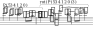
\includegraphics{sujeito-fugato}
    \label{fig:sujeito-fugato}
  }

  \subfloat[Contra-Sujeito]{
    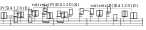
\includegraphics{contra-sujeito-fugato}
    \label{fig:contra-sujeito-fugato}
  }
  \caption{Elementos estruturais do fugato}
  \label{fig:elementos-fugato}
\end{figure}

O contra-sujeito é composto de três segmentos que contêm combinações
de operações de retrogradação e rotação de contornos (vide figura
\ref{fig:sujeito-fugato}). O primeiro segmento contém uma rotação de
fator 5 do retrógrado do contorno principal, resultando em (5 0 2 1 4
3). A primeira nota está elidida com a última nota do sujeito. O
segundo segmento contém uma rotação de fator 4 do retrógrado do
contorno principal---(3 5 0 2 1 4), e também está elidida ao segmento
anterior. Finalmente o terceiro segmento contém uma rotação de fator 3
do retrógrado do contorno principal---(4 3 5 0 2 1). Ao contrários dos
outros, ele não está elidido ao segmento anterior. Pode-se observar
que o contra-sujeito incorpora ainda uma sistemática nas suas
operações de contorno. A cada segmento o fator de rotação diminui em 1
ponto.

Do ponto de vista gestual, há uma passagem de uma menor densidade no
início da seção, com as entradas instrumentais sucessivas, para uma
maior densidade no final. Isto ocorre por três razões: (1) a entrada
da trompa em ritmo largo, (2) o estreitamento entre as entradas das
madeiras, e (3) a partir do compasso 128, o jogo de perguntas e
respostas com o primeiro segmento do sujeito, que ocorre entre as
duplas flauta e fagote versus oboé e clarinete.

A quinta seção contém um ostinato na linha do fagote em toda sua
extensão. Este ostinato é inspirado em um conhecido toque do jogo da
capoeira\footnote{A utilização deste elemento foi apenas pontual. Por
  este motivo não aprofundaremos em maiores explicações sobre a
  capoeira.}. Contornos não são usados de forma ortodoxa neste
ostinato, mas a idéia de $INT_1P$, ou seja (- + - + -), é sugerida
pelo movimento das notas $G$ e $A$.

Nesta seção a bifonia (vide figura \ref{fig:bifonia}) é apresentada em
sua forma mais explícita. Inicialmente na região grave, pelo clarinete
e pela trompa (comp. 137--144), depois brevemente entre oboé e trompa
(comp. 146--149), e mais adiante entre flauta e clarinete
(comp. 157--172).

Nesta seção contornos têm um papel especial na construção das
anacruze. A linha do oboé contém 3 anacruzes entre os compassos 149 e
156 (vide figura \ref{fig:anacruze-oboe}). A primeira delas
(comp. 149), um motivo utilizado nas seções seguintes, é um retrógrado
do motivo principal e mantém sua mesma estrutura de intervalos. A
segunda (comp. 151) é uma expansão intervalar da anacruze anterior que
transforma os intervalos de segunda em intervalos de terça. Já a
terceira anacruze (comp. 156), embora não seja verdadeiramente uma
anacruze por estar arrematando a melodia do oboé, pode ser entendida
como o início da bifonia posterior das linhas da flauta e
clarinete. Esta terceira anacruze é uma expansão da primeira anacruze
que transforma os intervalos de segunda em intervalos de quarta.

%% inserir análise no inkscape
\begin{figure}
  \centering
  \includegraphics{anacruze-oboe}
  \caption{Anacruze da linha do oboé}
  \label{fig:anacruze-oboe}
\end{figure}

Este trecho da linha do oboé é introduzido com a primeira anacruze,
arrematado pela terceira, e tem a segunda anacruze como uma operação
de preenchimento entre os dois segmentos do primeiro contorno.

%% falar sobre o gestual da quinta seção e uso da anacruze e da
%% semelhança com o contraponto da primeira seção

A sexta seção da obra, em contraste às anteriores, é caracterizada por
grupos de notas curtas, rápidas e desligadas. Estes grupos são
separados entre si por silêncios. As linhas dos instrumentos contêm
cada uma o motivo principal da peça modificado por operações de
rotação. Os grupos de notas curtas não englobam necessariamente todas
as notas do motivo modificado. Por vezes o silêncio interrompe o
motivo, como nos na linha da flauta, nos compassos 177--178 por
exemplo (vide figura \ref{fig:grupos-separados-silencio}).

\begin{figure}
  \centering
  \includegraphics{flauta-grupos-silencio}
  \caption{Grupos de notas separados por silêncios}
  \label{fig:grupos-separados-silencio}
\end{figure}

A linha da flauta contém o motivo principal em sua forma original. A
linha do clarinete contém uma rotação de fator 2 e uma expansão de
intervalos de segunda para intervalos de terça. A linha do oboé contém
um desvio da estrutura do contorno. Trata-se de uma rotação de fator 3
do motivo principal, porém com transposição da segunda metade do
motivo para uma oitava abaixo. Neste ponto a estrutura do contorno foi
sacrificada em prol do desenho gestual da seção, que não supera o
$D\sharp$4 neste trecho. Finalmente a linha do fagote contém uma
rotação de fator 4 do motivo principal e expansão semelhante ao do
clarinete. Na figura \ref{fig:notas-curtas-madeiras} estão exibidas
estas variações do motivo principal em cada elemento, na tabela
\ref{tab:operacoes-secao-6} há um esquema com as operações utilizadas
nestas variações, e na figura \ref{fig:rotacoes-534120} estão
representações gráficas das rotações utilizadas.

\begin{figure}
  \centering
    \includegraphics{notas-curtas-madeiras}
    \caption{Operações de rotação e expansão do motivo principal na 6ª
    seção}
  \label{fig:notas-curtas-madeiras}
\end{figure}

\begin{figure}
  \centering
  \subfloat[Rotação 2: (4 1 2 0 5 3)]{
    \includegraphics{c-412053}
    \label{fig:412053}  
  }
  \subfloat[Rotação 3: (1 2 0 5 3 4)]{
    \includegraphics{c-120534}
    \label{fig:120534}  
  }
  \subfloat[Rotação 4: (2 0 5 3 4 1)]{
    \includegraphics{c-205341}
    \label{fig:205341}  
  }
  \caption{Rotações no contorno (5 3 4 1 2 0)}
  \label{fig:rotacoes-534120}
\end{figure}

\begin{table}
  \centering
  \begin{tabular}{r|cc}
    Instrumento & Fator de rotação & Expansão \\
    \hline
    Flauta & 0 & Não \\
    Oboé & 3 & Não \\
    Clarinete & 2 & Sim \\
    Fagote & 4 & Sim \\
  \end{tabular}
  \caption{Operações na sexta seção}
  \label{tab:operacoes-secao-6}
\end{table}

Esta seção tem dois gestos interligados delineados. O primeiro gesto
(comp. 173--198) é marcado pelo aumento da densidade, obtido pela
diminuição dos silêncios. O colorido melódico tem destaque no final
deste gesto (comp. 194--198). O segundo gesto (comp. 199--214) é
caracterizado por graduais movimentos ascendentes e movimentação do
âmbito do grave para o agudo. A linha da trompa (comp. 206--215),
derivada da linha do oboé (comp. 149--157) interliga esta seção com a
seguinte.

A sétima e última seção engloba elementos importantes das seções
anteriores. A linha do fagote é uma repetição da quarta seção. A linha
do clarinete representa o ritmo e acentuação da terceira seção. A
linha da trompa representa o solo do fagote do início da peça. As
linhas do oboé e flauta representam a bifonia apresentada na quinta
seção. Finalmente o material apresentado pela flauta e oboé a partir
do compasso 239 representa o sujeito do fugato da quarta seção. As
relações de contornos nesta seção são, portanto, as mesmas que estes
citados elementos mantêm nas seções anteriores.

\subsection{Contornos associados a outros parâmetros musicais}
\label{sec:cont-assoc-outr}

Contornos estão associados a outros parâmetros musicais como
andamento, densidade e textura.

Os andamentos utilizados na peça---82, 66, 120, 108 e 112 (vide tabela
\ref{tab:secoes-obra}, p. \pageref{tab:secoes-obra})---representam o
contorno A(1 0 4 2 3). Este contorno é um subconjunto de 5 elementos
do contorno principal utilizado, \contpr{}.

Na seção inicial da obra relações de contornos estão associados a
densidade. A densidade neste trecho tem contorno D(1 3 2 5 4), isto é
começa com um instrumento, depois um trio, um duo, o quinteto completo
e um quarteto. Esta seção é iniciada com um solo de fagote (1) seguido
de um trio com fagote, clarinete e oboé (3). Ocorre então um duo entre
clarinete e flauta (2), um \eng{tutti} (5) e finalmente um quarteto
sem o fagote (4). Este contorno D é o retrógrado de um subconjunto de
5 elementos do contorno principal P.

As texturas presentes na peça podem ser divididas em dois grandes
grupos: de texturas homofônicas, que engloba texturas corais e de
melodia acompanhada; e de texturas polifônicas, que engloba textura
contrapontística e textura complexa. Estes grupos são apresentados
nesta ordem:
polifonia-homofonia-polifonia-homofonia-polifonia-homofonia. Considerando
que uma textura polifônica é mais complexa que uma textura homofônica,
a alternância entre estas texturas delineia um contorno de $INT_1$ (-
+ - + -), derivado do contorno principal \contpr{}.

\subsection{Operações de contorno não utilizadas}
\label{sec:oper-de-cont}

Nem todas as operações das teorias de contornos foram utilizadas na
composição. A \tr{COM-matrix}, por exemplo, é bastante utilizada para
análise, mas não encontramos uma forma interessante de usá-la na
composição.

\begin{figure}
  \centering
  \begin{tabular}{r|cccccc}
      & 5 & 3 & 4 & 1 & 2 & 0 \\
      \hline
    5 & 0 & - & - & - & - & - \\
    3 & + & 0 & + & - & - & - \\
    4 & + & - & 0 & - & - & - \\
    1 & + & + & + & 0 & + & - \\
    2 & + & + & + & - & 0 & - \\
    0 & + & + & + & + & + & 0
  \end{tabular}
  \caption{Matriz de comparação do contorno (5 3 4 1 2 0)}
  \label{fig:matriz-534120}
\end{figure}

\chapter{Conclusão}
\label{cha:conclusao}
